\begin{enumerate}[label=\thesection.\arabic*.,ref=\thesection.\theenumi]
\numberwithin{equation}{enumi}
\item Plot the polar plot of 
\begin{align}
G(s) = \frac{100(s+5)}{s(s+3)(s^2+4)}. 
\end{align}

\solution
To plot polar plot,we need to find magnitude and phase of frequency response for different values of $\omega$ from  0 to   $\infty$.

\begin{figure}[!h]
  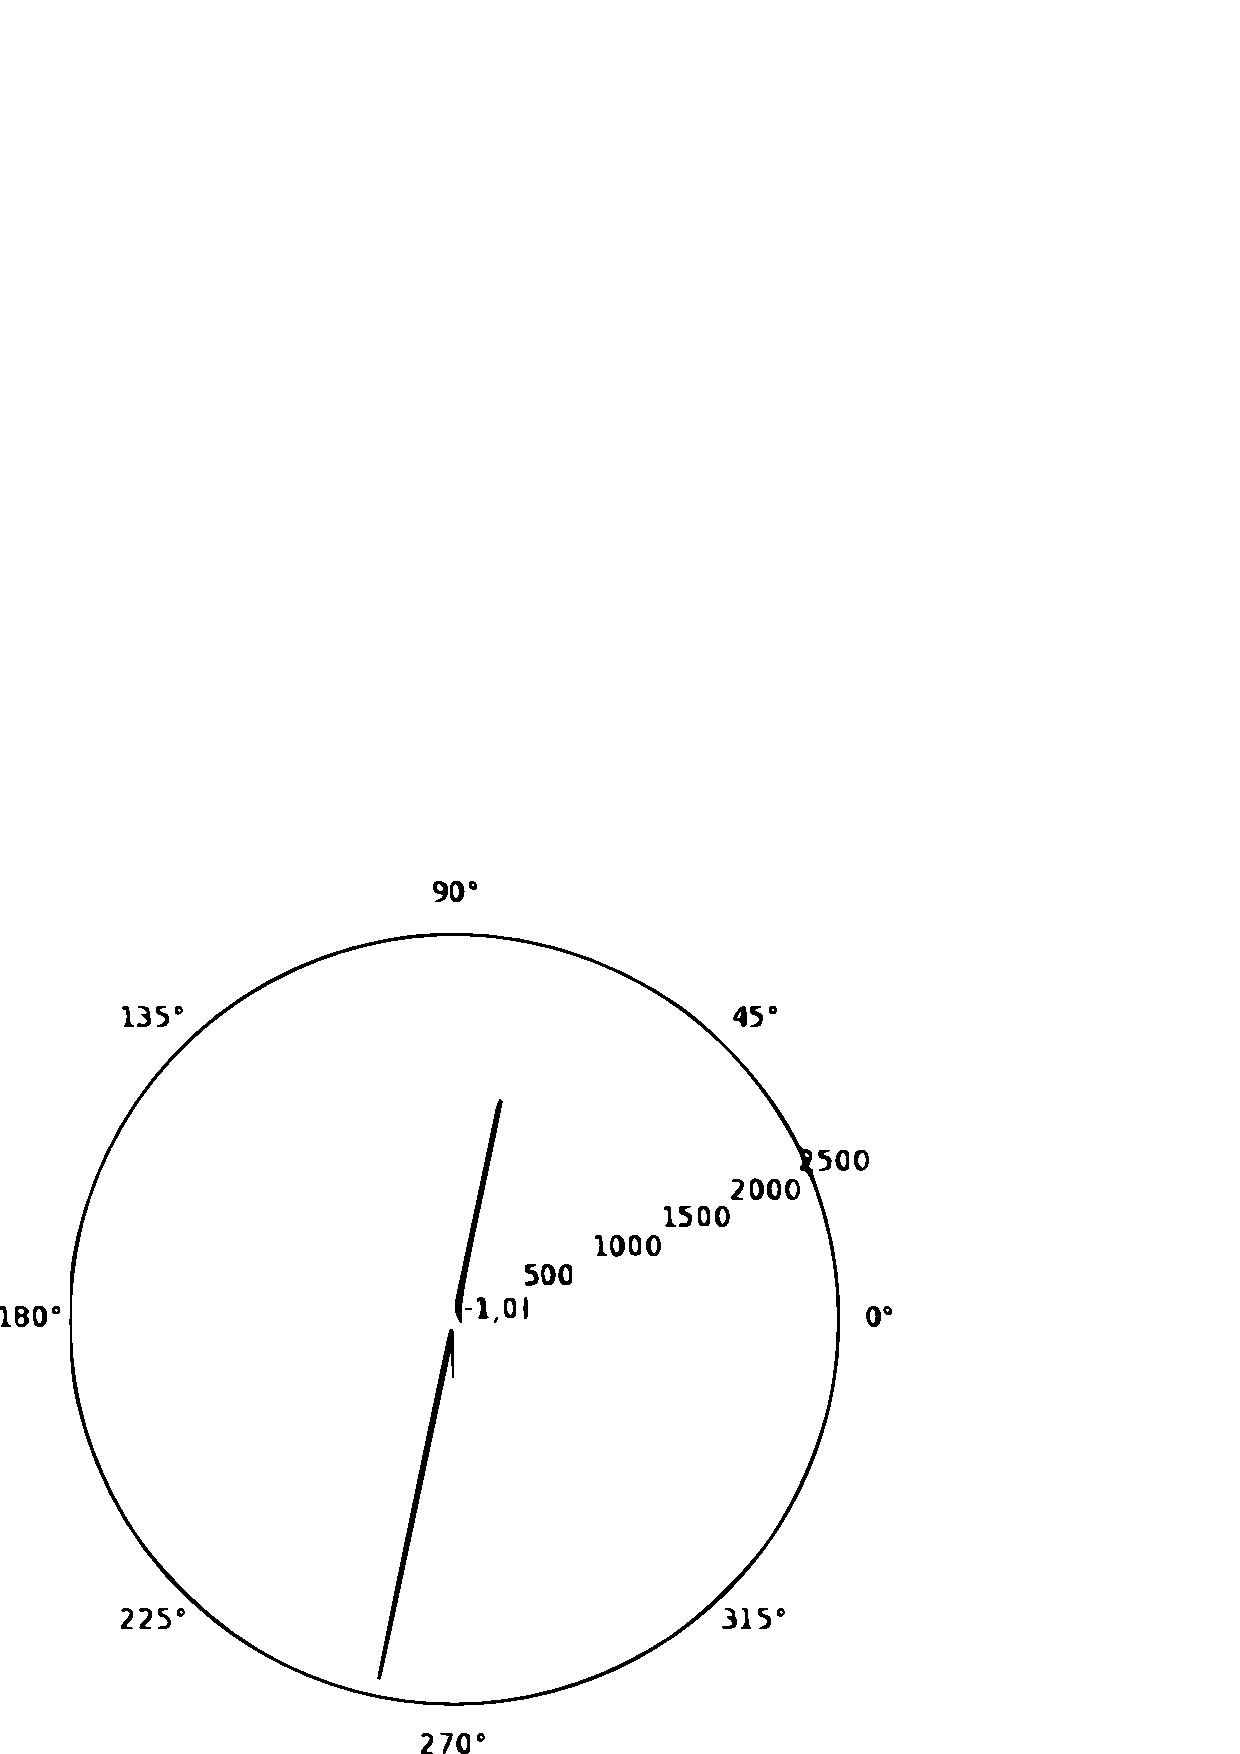
\includegraphics[width=\columnwidth]{ee18btech11042.png}
  \label{fig:polarplot}
\end{figure}

The following python code generates the polar plot : 
\begin{lstlisting}
codes/ee18btech11042.py
\end{lstlisting}
\item From polar plot we can find the stability of system and polar plots are drawn for open loop transfer functions.
\item
Stability is determined by position of point (-1,0) w.r.t to polar plot


\item If (-1,0)  is  on the left side  of the polar plot then the closed loop system is stable.
\item If (-1,0) is  on the right side of the polar plot then the closed loop system is unstable.
\item If t(-1,0) is on the polar plot then the closed loop system is marginally stable.
\item
Since (-1,0) is on the  polar plot the  above system is  marginally stable.

\end{enumerate}


